\ylDisplay{Küünlaleek} % Ülesande nimi
{Autor} % Autor
{lõppvoor} % Voor
{2012} % Aasta
{P 1} % Ülesande nr.
{1} % Raskustase
{
% Teema: Valgusõpetus
\ifStatement
Kõrgusega $h = 3,0$ cm küünlaleegi ja ekraani vahele paigutatakse õhuke kumerlääts nii, et ekraanile tekib leegi terav kujutis kõrgusega $h_1 = 6,0$ cm. Pärast läätse mõningat liigutamist tekkis ekraanile taas leegi terav kujutis. Leidke selle kõrgus $h_2$ nüüd.
\fi
\ifHint
Kui ese asub kaugusel $a$ läätsest ja tema tegelik kujutis kaugusel $b$ sellest, siis kiirte pööratavuse printsiibi kohaselt kui lääts paigutada kaugusele $b$ esemest, tekib tegelik kujutis kaugusele $a$ läätsest.
\fi
\ifSolution
Kui ese asub kaugusel $a$ läätsest ja tema tegelik kujutis kaugusel $b$ sellest, siis kiirte pööratavuse printsiibi kohaselt kui lääts paigutada kaugusele $b$ esemest, tekib tegelik kujutis kaugusele $a$ läätsest. Esimesel juhul on läätse suurendus $\frac{h_1}{h}= \frac{b}{a}$. Teisel juhul $\frac{h_2}{h}= \frac{a}{b} = \frac{h}{h_1}$, millest $h_2 = \frac{h_2}{h_1} = 1,5$ cm.
\begin{center}
	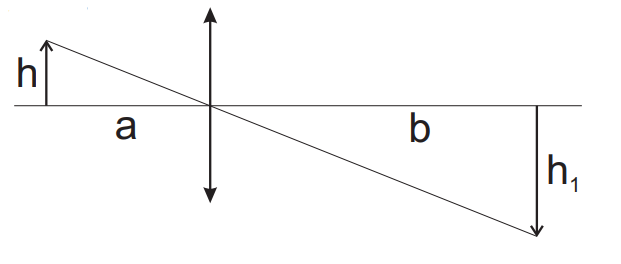
\includegraphics[width=0.5\linewidth]{2012-v3p-01-lah.PNG}
\end{center}
\fi
}